\section{Exercise eight}

The system comprises three modules (A, B, and C) and is designed to function correctly if both A and B operate correctly or if C operates correctly.
The availabilities of the modules are as follows: $A_{\text{A}} = 0.97$, $A_{\text{B}} = 0.92$, and $A_{\text{D}} = 0.95$.
\begin{enumerate}
    \item Illustrate the reliability block diagram of the system.
    \item Compute the system's availability.
\end{enumerate}

\subsection*{Solution}
\begin{enumerate}
    \item The reliability block diagram of the system is depicted below:
        \begin{figure}[H]
            \centering
            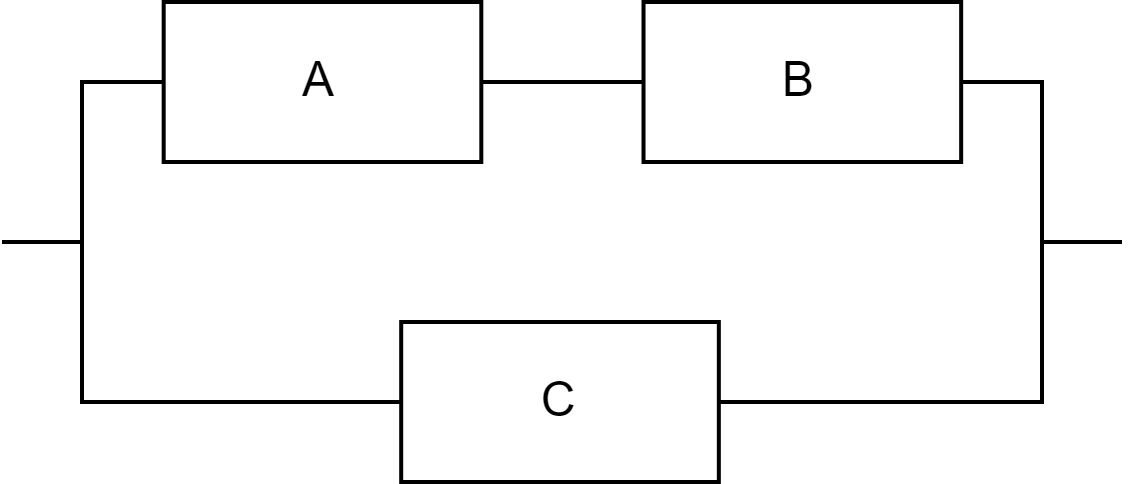
\includegraphics[width=0.5\linewidth]{images/rbd1.png}
        \end{figure}
    \item To calculate the availability of the system, we first determine the availability of blocks A and B in series:
        \[A_{\text{AB}}=A_{\text{A}}A_{\text{B}}=0.97\cdot 0.92=0.89\]
        Subsequently, with block AB in parallel with C, the overall availability becomes:
        \[A_{s}=1-\left(1-A_{\text{AB}}\right)\left(1-A_{\text{C}}\right)=1-(0.11)(0.04)=0.9956\]
\end{enumerate}